\chapter{Projekt symulatora operacji antyterrorystycznych}
\section{Model obiektowy}
Wykorzystywany podczas implementacji Javascript, jako skryptowy język programowania, nie jest językiem ściśle obiektowym (jak np. Java), lecz mimo wszystko umożliwia on pisanie aplikacji technikami programowania obiektowego. Do tego celu służy m. in. prototypowanie, które pozwala także na dziedziczenie przygotowywanych klas.

W grze symulacyjnej, będącej przedmiotem tej pracy dyplomowej, możemy wyróżnić trzy obiekty, które wywodzą się bezpośrednio z klasy obiektu javascriptowego oraz dziesięć klas, które dziedziczą atrybuty i metody z różnych klas kształtów, zawartych w bibliotece Kinetic.js. Nazwy metod, które są postrzegane jako prywatne dla danej klasy, rozpoczynają się od znaku podkreślenia "\_"\footnote{w Javascript'cie nie ma dedykowanego mechanizmu rozróżniania metod prywatnych i publicznych}. W prezentowanych tabelach zostały pominięte atrybuty i metody odziedziczone z innych klas. Definicje klas wchodzących w skład biblioteki Kinetic.js można znaleźć na stronie projektu\cite{kineticPage}.

Obiekt \textbf{Game} zawiera informacje dotyczące świata gry, tj. jego wymiarów, aktualnej konfiguracji oraz funkcjonujących jednostek. Stanowi on interfejs dla obiektów innych klas, przez który mogą one dostrzegać zmiany zachodzące w świecie gry. Metody zawarte w obiekcie Game pozwalają ma kontrolowanie symulacji. Opis atrybutów oraz zaimplementowanych metod znajduje się w tabeli \ref{objectsGame}.

\begin{table}
\begin{center}
\begin{tabular}{|p{0.28\textwidth}|p{0.72\textwidth}|}
\hline
\textbf{Game} & Opis\\\hline		
	width & szerokość sceny wyrażona w pikselach\\
	height & wysokość sceny wyrażona w pikselach\\
	mapDensity & wymiar jednego kafelka na mapie, na potrzeby reprezentacji grafowej\\
	uiState & aktualny stan interfejsu graficznego, określa która strona konfiguracji jest aktualnie otwarta\\
	stage & obiekt sceny zawierający poszczególne warstwy\\
	map & obiekt mapy zawierający część informacji o konfiguracji\\ 
	entities & warstwa sceny zawierająca istniejące w symulacji jednostki (terroryści i antyterroryści)\\
	configObjects & warstwa sceny zawierająca obiekty wspomagające konfigurację (szkic punktu kluczowego, szkic punktu startowego itp.)\\
	mapObjects & warstwa sceny zawierająca obiekty należące do mapy (ściany, punkty kluczowe itp.)\\
	paused & zmienna logiczna informująca o włączeniu/wyłączeniu pauzy\\
	antiterroristsCount & liczba antyterrorystów wynikająca z konfiguracji\\
	terroristsCount & liczba terrorystów wynikająca z konfiguracji\\
	keypointIndex & numer aktualnie realizowanego punktu kluczowego przez antyterrorystów
\\\hline
	init & inicjalizuje aplikację tworząc scenę oraz warstwy\\
	initMap & tworzy obiekt mapy\\
	togglePause & przyłącza stan pauzy\\
	startGame & rozpoczyna symulację\\ 
	endGame & kończy symulację\\
	getEntities & zwraca listę wszystkich jednostek istniejących w bieżącej symulacji\\
	getAliveTerrorists & zwraca listę niezabitych terrorystów w bieżącej symulacji\\ 
	getAliveAntiterrorists & zwraca listę niezabitych antyterrorystów w bieżącej symulacji\\
	checkAliveEntities & sprawdza stan jednostek, a w razie zaistnienia zamknięcia konfliktu, tworzy odpowiedni wpis w logach\\
	getNodeByPosition & zwraca węzeł w grafie na podstawie zadanych współrzędnych\\
	\_spawnTerrorists & tworzy obiekty terrorystów podczas startu symulacji\\ 
	\_spawnAntiterrorists & tworzy obiekty antyterrorystów podczas startu symulacji
\\\hline
\end{tabular}
\caption {Obiekt gry - Game\label{objectsGame}}
\end{center}
\end{table} 

Obiekt \textbf{GameControl} zawiera przede wszystkim metody, które wiążą interfejs z~obiektem Game. Są tutaj zdefiniowane wszystkie metody wywoływane poprzez kliknięcia użytkownika w przyciski znajdujące się na interfejsie. Opis atrybutów oraz zaimplementowanych metod znajduje się w tabeli \ref{objectsGameControl}. 

\begin{table}
\begin{center}
\begin{tabular}{|p{0.28\textwidth}|p{0.72\textwidth}|}
\hline
\textbf{GameControl} & Opis\\\hline		
	storagePrefix & stała zawierająca informację o prefiksie dla nazw zapisywanych konfiguracji\\
	simStartTime & czas rozpoczęcia symulacji wyrażony w milisekundach\\
	winMessage & wiadomość o ew. zwycięstwie jednej ze stron konfliktu
\\\hline
	init & inicjalizuje interfejs, tworzy powiązania z obiektem Game\\
	log & umieszcza wpis o zadanym tekście w logach\\
	setWinMessage & tworzy wiadomość dotyczącą zwycięstwa jednej ze stron konfliktu\\
	configs & zwraca listę wcześniej zapisanych konfiguracji\\
	loadConfig & wczytuje wybraną konfigurację\\
	saveConfig & zapisuje bieżącą konfigurację\\
	removeConfig & usuwa wybraną konfigurację\\
	startSim & powiązana z przyciskiem rozpoczynającym symulację \\
	pauseSim & powiązana z przyciskiem wstrzymującym symulację\\ 
	stopSim & powiązana z przyciskiem zatrzymującym symulację\\ 
	removeLastWall & powiązana z przyciskiem usuwającym ostatnio utworzoną ścianę\\
	clearWalls & powiązana z przyciskiem usuwającym wszystkie ściany\\
	removeSpawnZone & powiązana z przyciskiem usuwającym punkt startowy / końcowy dla antyterrorystów\\
	removeLastKeypoint & powiązana z przyciskiem usuwającym ostatnio utworzony punkt kluczowy\\
	clearKeypoints & powiązana z przyciskiem usuwającym wszystkie punkty kluczowe\\
	nextConfig & otwiera następną stronę konfiguracji\\
	previousConfig & otwiera poprzednią stronę konfiguracji\\
	changeUiState & otwiera zadaną stronę konfiguracji\\
	clearEntitiesList & usuwa dane jednostek ze statystyk\\
	createEntitiesList & dodaje dane jednostek do statystyk\\
	updateStat & aktualizuje statystyki dla danej jednostki\\
	\_updateCursor & zmienia styl kursora myszy nad sceną\\
	\_updateNumberData & zmienia dane liczbowe o jednostkach w obiekcie Game\\
	\_updateConfigStatus & zwraca informację o ew. niekompletnej konfiguracji 
\\\hline
\end{tabular}
\caption {Obiekt kontroli gry - GameControl\label{objectsGameControl}}
\end{center}
\end{table} 

Obiekt \textbf{Sounds} zawiera definicję ścieżek do plików dźwiękowych wykorzystywanych w grze oraz metody pozwalające je odtwarzać i zatrzymywać. W grze symulacyjnej zdefiniowane są trzy dźwięki: dźwięk rozpoczynający symulację, wystrzały terrorystów oraz wystrzały antyterrorystów. Opis atrybutów oraz zaimplementowanych metod znajduje się w tabeli \ref{objectsSounds}. 

\begin{table}
\begin{center}
\begin{tabular}{|p{0.28\textwidth}|p{0.72\textwidth}|}
\hline
\textbf{Sounds} & Opis\\\hline		
	list & tablica asocjacyjna zawierająca ścieżki do plików dźwiękowych\\
	instances & tablica asocjacyjna zwierająca instancje odgrywanych plików dźwiękowych
\\\hline
	init & tworzy powiązanie z obiektem Game\\
	play & rozpoczyna odtwarzanie danego dźwięku\\
	stop & zatrzymuje odtwarzanie danego dźwięku
\\\hline
\end{tabular}
\caption {Obiekt dźwięków gry - Sounds\label{objectsSounds}}
\end{center}
\end{table} 

Obiekt klasy \textbf{Game.Map} rozszerza klasę Kinetic.Rect. Zawiera on referencje do elementów konfiguracji symulacji - ściany, punkty kluczowe. Ponadto obiekt mapy zawiera graf reprezentujący stan poszczególnych pól na mapie (zajęte lub niezajęte), co jest potrzebne podczas generowania ścieżek dla poruszających się jednostek. Obiekt mapy posiada także metody pozwalające na serializowanie konfiguracji do formatu JSON\footnote{JavaScript Object Notation - tekstowy format wymiany danych, alternatywa dla XML} oraz do importu konfiguracji dostarczonej w takim formacie. Obsługa zdarzeń nad sceną, których źródłem jest urządzenie wskazujące, jest również zaimplementowana na obiekcie mapy. Opis atrybutów oraz zaimplementowanych metod znajduje się w tabeli \ref{objectsGameMap}.  

\begin{table}
\begin{center}
\begin{tabular}{|p{0.28\textwidth}|p{0.72\textwidth}|}
\hline
\textbf{Game.Map} & Opis\\\hline		
	newWall & obiekt szkicu tworzonej ściany\\
	graph & obiekt grafu, niezbędnego do wytyczania ścieżek\\
	zone & obiekt punktu startowego / końcowego antyterrorystów\\
	zoneDraft & obiekt szkicu punktu startowego / końcowego antyterrorystów\\
	newKeypoint & obiekt szkicu punktu kluczowego\\
	walls & tablica zawierająca istniejące ściany\\
	keypoints & tablica zawierająca istniejące punkty kluczowe
\\\hline
	init & inicjalizuje obiekt mapy\\ 
	removeLastWall & usuwa ostatnio utworzoną ścianę\\
	clearWalls & usuwa wszystkie ściany\\
	removeLastKeypoint & usuwa ostatnio utworzony punkt kluczowy\\
	clearKeypoints & usuwa wszystkie punkty kluczowe\\
	removeZone & usuwa punkt startowy / końcowy antyterrorystów\\
	serializeConfig & serializuje bieżącą konfigurację\\
	importConfig & deserializuje dostarczoną konfigurację i tworzy nowe obiekty na jej podstawie\\
	\_bindEvents & inicjalizuje obsługę zdarzeń nad sceną\\
	\_buildGraph & inicjalizuje graf\\
	\_buildGrid & buduje siatkę nad sceną\\
	\_initWall & inicjalizuje nową ścianę\\
	\_updateWall & uaktualnia obiekt szkicu ściany\\
	\_addWall & dodaje utworzoną ścianę do listy ścian\\
	\_updateWallOnGraph & oznacza węzły grafu, które pokrywa zadana ściana\\
	\_buildZoneDraft & inicjalizuje punkt startowy / końcowy antyterrorystów\\
	\_buildKeypoint & inicjalizuje punkt kluczowy\\
	\_showDraftZone & pokazuje szkic punktu startowego / końcowego antyterrorystów gdy ukryty\\
	\_hideDraftZone & ukrywa szkic punktu startowego / końcowego antyterrorystów gdy widoczny\\
	\_setZone & ustanawia punkt startowy / końcowy antyterrorystów\\ 
	\_updateDraftZone & uaktualnia położenie szkicu punktu startowego / końcowego antyterrorystów \\
	\_addKeypoint & dodaje utworzony punkt kluczowy do listy punktów kluczowych\\
	\_showNewKeypoint & pokazuje szkic punktu kluczowego gdy ukryty\\ 
	\_hideNewKeypoint & ukrywa szkic punktu kluczowego gdy widoczny\\
	\_updateNewKeypoint & uaktualnia położenie szkicu punktu kluczowego 
\\\hline
\end{tabular}
\caption {Klasa mapy - Game.Map\label{objectsGameMap}}
\end{center}
\end{table} 


Klasa \textbf{Game.Line} rozszerza klasę Kinetic.Line. Sama stanowi podstawę dla klas Game.GridLine oraz Game.Wall. Klasa Game.Line zawiera metody sprawdzające przecięcia linii z inną linią oraz linii z okręgiem. Metody te są wykorzystywane w wielu metodach należących do obiektów ruchomych (klasa Game.Entity). Opis atrybutów oraz zaimplementowanych metod znajduje się w tabeli \ref{objectsGameLine}.   

\begin{table}
\begin{center}
\begin{tabular}{|p{0.45\textwidth}|p{0.55\textwidth}|}
\hline
\textbf{Game.Line} & Opis\\\hline		
	 & \emph{klasa ta zawiera wyłącznie atrybuty dziedziczone}
\\\hline
	init & inicjalizuje obiekt linii\\
	getStartPoint & zwraca współrzędne punktu początkowego linii\\
	getEndPoint & zwraca współrzędne punktu końcowego linii\\
	getVecStartPoint & zwraca punkt początkowy linii w postaci wektora\\
	getVecEndPoint & zwraca punkt końcowy linii w postaci wektora\\ 
	setStartPoint & ustawia punkt początkowy linii\\
	setEndPoint & ustawia punkt końcowy linii\\
	getIntersectionPointWithLine & zwraca współrzędne punktu przecięcia dwóch linii\\
	getVecIntersectionPointWithSphere & zwraca punkt przecięcia linii i okręgu w postaci wektora\\
	getVecIntersectionPoint & zwraca punkt przecięcia dwóch linii w postaci wektora\\
	getNormals & zwraca wektory normalne dla danej linii\\
	\_getClosestPointOnLine & zwraca najbliższy punkt na linii do zadanego punktu 
\\\hline
\end{tabular}
\caption {Klasa linii - Game.Line\label{objectsGameLine}}
\end{center}
\end{table} 

Klasa \textbf{Game.Wall} rozszerza klasę Game.Line. Instancje tej klasy reprezentują ściany w grze symulacyjnej. Klasa zawiera dodatkowo metodę sprawdzającą poprawność budowanej ściany, która musi być linią poziomą lub pionową, a nie może być linią skośną. Ściany w grze stanowią dla jednostek jedyną przeszkodę, którą jednostki muszą omijać. Utworzone ściany mają swoje odzwierciedlenie na grafie w postaci niedostępnych dla jednostek węzłów. Opis atrybutów oraz zaimplementowanych metod znajduje się w tabeli \ref{objectsGameWall}. 

\begin{table}
\begin{center}
\begin{tabular}{|p{0.28\textwidth}|p{0.72\textwidth}|}
\hline
\textbf{Game.Wall} & Opis\\\hline		
	valid & zawiera informację czy ściana jest poprawna
\\\hline
	init & inicjalizuje obiekt ściany\\
	setEndPoint & nadpisana metoda klasy Game.Line, dodatkowo wywołuje metodę \_validate\\
	isVertical & zwraca informację czy linia jest pionowa\\
	isHorizontal & zwraca informację czy linia jest pozioma\\
	\_validate & sprawdza poprawność zbudowanej linii
\\\hline
\end{tabular}
\caption {Klasa ściany - Game.Line\label{objectsGameWall}}
\end{center}
\end{table} 

Klasa \textbf{Game.Keypoint} rozszerza klasę Kinetic.Text. Instancje tej klasy reprezentują punkty kluczowe w grze symulacyjnej. Klasa zawiera metodę sprawdzającą poprawność tworzonego punktu kluczowego, który nie może leżeć w miejscu gdzie jest ściana. Podczas rozpoczynania symulacji, terroryści są tworzeni w losowo wybranych punktach kluczowych. Punkty te jednocześnie wytyczają trasę jaką muszą pokonać antyterroryści podczas przeprowadzanego szturmu. Antyterrorysta lider, po dotarciu do danego punktu kluczowego, wytycza bezkolizyjną ścieżkę do kolejnego punktu. Opis atrybutów oraz zaimplementowanych metod znajduje się w tabeli \ref{objectsGameKeypoint}. 

\begin{table}
\begin{center}
\begin{tabular}{|p{0.28\textwidth}|p{0.72\textwidth}|}
\hline
\textbf{Game.Keypoint} & Opis\\\hline		
	valid & zawiera informację czy punkt kluczowy jest poprawny
\\\hline
	init & inicjalizuje obiekt punktu kluczowego\\
	updatePosition & uaktualnia położenie punktu kluczowego\\
	\_validate & sprawdza poprawność tworzonego punktu kluczowego
\\\hline
\end{tabular}
\caption {Klasa punktu kluczowego - Game.Keypoint\label{objectsGameKeypoint}}
\end{center}
\end{table} 

Klasa \textbf{Game.Entity} rozszerza klasę Kinetic.Image. Sama stanowi podstawę dla klas Game.Terrorist, Game.Antiterrorist oraz Game.Bullet. Klasa ta posiada metody pozwalające wyliczać wektor prędkości dla algorytmów poruszania się oraz sprawdzać kolizję z innymi obiektami. Część atrybutów i metod jest tutaj odpowiedzialna za realizację wspólnych dla terrorystów i antyterrorystów taktyk. Dzięki implementacji metody \emph{update}, położenie obiektów na scenie jest stale aktualizowane. Opis atrybutów znajduje się w tabeli \ref{objectsGameEntityAttrs}, natomiast opis zaimplementowanych metod znajduje się w tabeli \ref{objectsGameEntityFuncs}. 

\begin{table}[p]
\begin{center}
\begin{tabular}{|p{0.28\textwidth}|p{0.72\textwidth}|}
\hline
\textbf{Game.Entity} & Opis atrybutów\\\hline		
    imageSrc & ścieżka do pliku z reprezentacją graficzną\\
    maxSpeed & maksymalna prędkość obiektu\\
    velX & współrzędna X wektora prędkości\\
    velY & współrzędna Y wektora prędkości\\
    tarX & współrzędna X celu\\
    tarY & współrzędna Y celu\\
    rayLine & obiekt linii, która sprawdza możliwość wystąpienia kolizji\\
    groupIndex & numer obiektu w danej stronie konfliktu\\
    isAlive & zawiera informację czy obiekt żyje\\
    dieAlpha & stopień przezroczystości, jaka jest stosowana, gdy obiekt ginie\\
    speed & aktualna prędkość\\
    avoidDistance & dystans, jaki obiekt powinien zachowywać od kolidujących obiektów\\
    lookAhead & długość linii, sprawdzającej możliwość wystąpienia kolizji\\
    arrivePrecision & dokładność, z jaką się określa czy obiekt dotarł do celu\\
    targetEntity & obiekt ruchomy, który jest aktualnym celem\\
    watchedEntity & obiekt ruchomy, który jest obserwowany, ale nie atakowany\\
    healthPoints & liczba punktów życia\\
    healthPointsMax & liczba punktów życia, jakie obiekt posiada po utworzeniu\\
    collisionRadius & promień okręgu wytyczającego strefę kolizyjną obiektu\\
    kills & liczba zabić dokonanych przez obiekt\\
    nodeIndex & indeks aktualnie odwiedzanego węzła na ścieżce\\
    path & ścieżka reprezentowana przez tablicę węzłów\\
    currentState & nazwa aktualnego stanu obiektu\\
    checkLocationTimeMax & maksymalny czas, jaki może zostać poświęcony na sprawdzenie lokacji\\
    checkLocationTime & aktualny czas, jaki pozostał na sprawdzenie lokacji\\
    sightDistance & zasięg wzroku obiektu\\
    name & nazwa typu obiektu\\
    enemyName & nazwa wrogiego typu obiektu
\\\hline
\end{tabular}
\caption {Atrybuty klasy obiektu ruchomego - Game.Entity\label{objectsGameEntityAttrs}}
\end{center}
\end{table} 

\begin{table}
\begin{center}
\begin{tabular}{|p{0.34\textwidth}|p{0.66\textwidth}|}
\hline
\textbf{Game.Entity} & Opis metod\\\hline		
	init & inicjalizuje obiekt ruchomy\\
	setTarget & ustawia cel wg zadanych współrzędnych\\
	setTargetEntity & ustawia inny obiekt jako swój cel\\
	currentTargetEntity & zwraca aktualny obiekt będący celem\\
	unsetTargetEntity & usuwa przypisanie celu, który jest obiektem\\
	updateTargetEntity & uaktualnia wiedzę o położeniu celu\\
	setVelocity & ustawia wektor prędkości\\
	hasVelocity & zwraca informację czy obiekt się porusza\\
	getVecPosition & zwraca aktualną pozycję w postaci wektora\\
	getVecVelocity & zwraca aktualną prędkość w postaci wektora\\
	getVecTarget & zwraca aktualną pozycję celu w postaci wektora\\
	update & przesuwa obiekt o zadany wektor prędkości oraz aktualizuje orientację\\
	changeState & zmienia stan obiektu na zadany\\
	die & uśmierca obiekt\\
	setRandomPositionInCircle & wybiera losową pozycję obiektu wokół określonego okręgu\\
	isInCollision & sprawdza czy obiekt nie koliduje ze ścianą lub inną istniejącą jednostką\\
	seek & aktualizuje wektor prędkości w kierunku do celu\\
	flee & aktualizuje wektor prędkości w kierunku przeciwnym do celu\\
	stop & zatrzymuje obiekt\\
	arrived & sprawdza czy obiekt dotarł do celu\\
	checkForCollision & sprawdza czy obiekt nie koliduje ze ścianą\\
	closestSeenOpponent & zwraca najbliższego przeciwnika w zasięgu wzroku\\
	takeDamage & zadaje rany obiektowi poprzez odbiór punktów życia\\
	watchForEnemy & metoda pozwalająca na obserwowanie przeciwnika i po określonym czasie przejście do ataku\\
	attack & atakowanie przeciwnika poprzez oddawanie strzałów co określony interwał czasowy\\
	calculatePath & wyliczanie ścieżki do zadanego celu\\
	checkLocation & metoda pozwalająca na przejście po ścieżce do wcześniej wytyczonego celu\\
	setCheckLocation & metoda określająca cel, do którego należy dotrzeć wg wytyczonej ścieżki\\
	\_logDeath & tworzenie wpisu w logach o śmierci obiektu\\
	\_updateCollisionRay & uaktualnia położenie linii, która sprawdza możliwość wystąpienia kolizji\\
	\_calculateVelocity & wyliczanie wektora prędkości
\\\hline
\end{tabular}
\caption {Metody klasy obiektu ruchomego - Game.Entity\label{objectsGameEntityFuncs}}
\end{center}
\end{table} 

Klasa \textbf{Game.Antiterrorist} rozszerza klasę Game.Entity. Instancje tej klasy reprezentują antyterrorystów w grze symulacyjnej. Najważniejszą metodą zawartą w~tej klasie jest \emph{think}. Decyduje ona o działaniach antyterrorysty poprzez umożliwienie zmiany stanów. Opis atrybutów oraz zaimplementowanych metod znajduje się w tabeli \ref{objectsGameAntiterrorist}.

Klasa \textbf{Game.Terrorist} rozszerza klasę Game.Entity. Instancje tej klasy reprezentują terrorystów w grze symulacyjnej. Podobnie jak w klasie Game.Antiterrorist, kluczową rolę w tej klasie odgrywa metoda \emph{think}. Opis atrybutów oraz zaimplementowanych metod znajduje się w tabeli \ref{objectsGameTerrorist}. Dodatkowo w rozdziale \ref{tacticts} jest przedstawiony diagram przejść międzystanowych, który w ilustruje taktykę charakterystyczną dla działań antyterrorystów i terrorystów. 

\begin{table}
\begin{center}
\begin{tabular}{|p{0.28\textwidth}|p{0.72\textwidth}|}
\hline
\textbf{Game.Antiterrorist} & Opis\\\hline		
	reactionTimeMax & czas reakcji przejścia  z obserwowania do ataku\\
	reactionTime & aktualny czas pozostały do przejścia do ataku\\
	shootInterval & czas pomiędzy kolejnymi wystrzałami\\
	shootTime & aktualny czas pozostały do wystrzału\\
	followDistance & odległość, w jakiej antyterrorysta podąża za poprzednikiem\\
	isLeader & zawiera informację, czy antyterrorysta jest liderem\\
	keypointIndex & numer aktualnie realizowanego punktu kluczowego przez lidera antyterrorystów
\\\hline
	think & metoda odpowiedzialna za realizację taktyk\\
	followEntity & podążanie w linii za poprzednikiem\\ 
	followPath & podążanie do następnego punktu kluczowego po ścieżce\\
	followExtraction & podążanie do punktu startowego / końcowego antyterrorystów\\
	avoid & omijanie napotkanej ściany poprzez wytyczenie ścieżki\\
	changeToDefaultState & zmiana stanu do domyślnego (dla antyterrorystów jest to \emph{followEntity})\\
	\_reactOnDamage & reakcja na postrzał
\\\hline
\end{tabular}
\caption {Klasa antyterrorysty - Game.Antiterrorist\label{objectsGameAntiterrorist}}
\end{center}
\end{table} 


\begin{table}
\begin{center}
\begin{tabular}{|p{0.28\textwidth}|p{0.72\textwidth}|}
\hline
\textbf{Game.Terrorist} & Opis\\\hline		
	reactionTimeMax & czas reakcji przejścia  z obserwowania do ataku\\
	reactionTime & aktualny czas pozostały do przejścia do ataku\\
	shootInterval & czas pomiędzy kolejnymi wystrzałami\\
	shootTime & aktualny czas pozostały do wystrzału\\
	wanderCircleDistance & odległość środka okręgu wyznaczającego kurs wędrówki od terrorysty\\
	wanderRadius & promień okręgu wyznaczającego kurs wędrówki\\
	wanderRate & zakres wahania kierunku wędrówki\\
	wanderOrientation & orientacja kierunku wędrówki\\
	standingProbability & prawdopodobieństwo przejścia do stanu postoju\\
	standingTimeMax & maksymalny czas, jaki może trwać pojedynczy postój\\
	standingTime & czas pozostały do zakończenia aktualnego postoju
\\\hline
	think & metoda odpowiedzialna za realizację taktyk\\
	stand & metoda odpowiedzialna za sprawdzanie czy postój ma nadal trwać\\
	wander & poruszanie się zgodnie z kierunkiem wędrówki\\
	avoid & omijanie napotkanej ściany poprzez skierowanie terrorysty do punktu wyznaczanego przez normalną ściany\\
	changeToDefaultState & zmiana stanu do domyślnego (dla terrorystów jest to \emph{wander})\\
	\_wantToStand & sprawdzenie czy terrorysta na wykonać postój\\
	\_reactOnDamage & reakcja na postrzał
\\\hline
\end{tabular}
\caption {Klasa terrorysty - Game.Terrorist\label{objectsGameTerrorist}}
\end{center}
\end{table} 

Klasa \textbf{Game.Bullet} rozszerza klasę Game.Entity. Instancje tej klasy reprezentują pociski w grze symulacyjnej. Podczas przemieszczania się pocisku, sprawdzane jest czy nie trafił on w ścianę lub jednostkę. Symulowany odgłos wystrzału oraz trafienia może przyciągać uwagę terrorystów znajdujących się w określonej odległości od pocisku. Im dłużej pocisk się porusza, tym mniejszą posiada energię, która decyduje o ew. ranach zadanych jednostce. Opis atrybutów oraz zaimplementowanych metod znajduje się w tabeli \ref{objectsGameBullet}. 

\begin{table}
\begin{center}
\begin{tabular}{|p{0.30\textwidth}|p{0.70\textwidth}|}
\hline
\textbf{Game.Bullet} & Opis\\\hline		
	shooter & referencja do obiektu jednostki,  która wystrzeliła pocisk\\
	energy & energia, jaką aktualnie posiada pocisk\\
	bulletRange & zasięg pocisku\\	
	attentionRange & promień w jakim wystrzelony pocisk jest słyszalny
\\\hline
	move & metoda odpowiedzialna za ruch pocisku i sprawdzenie ew. trafienia\\
	\_drawTerroristsAttention & zmiana stanu terrorystów będących w zasięgu słyszalności wystrzału lub trafienia\\
	\_playSound & odtwarzanie dźwięku wystrzału
\\\hline
\end{tabular}
\caption {Klasa pocisku - Game.Bullet\label{objectsGameBullet}}
\end{center}
\end{table} 
\clearpage
Poza wymienionymi klasami, w grze symulacyjnej zdefiniowane są jeszcze klasy, które wyłącznie nadpisują konfigurację wyświetlania kształtu. Należą do nich:
\begin{itemize}
	\item Game.Zone - dziedziczy z klasy Kinetic.Circle. Instancje tej klasy reprezentują punkt startowy / początkowy antyterrorystów
	\item Game.GridLine - dziedziczy z klasy Kinetic.Line. Instancje tej klasy reprezentują siatkę narzuconą na scenę
\end{itemize}

\section{Opis algorytmów}
W tym rozdziale zostaną przedstawione wybrane algorytmy, jakie są wykorzystywane w grze symulacyjnej, będącej przedmiotem tej pracy dyplomowej. Słowny opis jest uzupełniony pseudokodami lub implementacją w języku Javascript.

\subsection{Myślenie i poruszanie się jednostek}
Antyterroryści i terroryści w grze symulacyjnej posiadają zaimplementowaną metodę \emph{think} pozwalającą na realizację działań zapisanych w konkretnych stanach (listing \ref{thinkAt} oraz \ref{thinkTer}). Prócz wywołania metod odpowiadającym konkretnym stanom, wywoływane są także metody \emph{watchForEnemy} oraz \emph{checkForCollision}. Ta pierwsza pozwala jednostce na obserwowanie otoczenia w poszukiwaniu przeciwników, natomiast druga na bezpieczne omijanie ścian. Metody odpowiadające za realizację poszczególnych stanów podejmują najczęściej decyzję, gdzie leży następny cel jednostki.

\begin{table}
\begin{center}
\begin{lstlisting}
    think: function(){
        this.watchForEnemy();
        switch(this.currentState) {
            case 'idle': break;
            case 'init': this.setup(); break;
            case 'follow entity': this.followEntity(); break;
            case 'follow path': this.followPath(); break;
            case 'follow extraction': this.followExtraction(); break;
            case 'check location': this.checkLocation(); break;
            case 'attack': this.attack(); break;
            default: this.changeToDefaultState(); break;
        }
        if (this.avoiding) this.wanderOrientation = this.getRotation();
        this.avoiding = this.checkForCollision();
    }
 \end{lstlisting}
\caption {Metoda think w klasie Game.Antiterrorist}
\label{thinkAt}
\end{center}
\end{table}

\begin{table}
\begin{center}
\begin{lstlisting}
    think: function(){
        this.watchForEnemy();
        switch(this.currentState) {
            case 'idle': break;
            case 'init': this.setup(); break;
            case 'stand': this.stand(); break;
            case 'wander': this.wander(); break;
            case 'check location': this.checkLocation(); break;
            case 'attack': this.attack(); break;
            default: this.changeToDefaultState(); break;
        }
        if (this.avoiding) this.wanderOrientation = this.getRotation();
        this.avoiding = this.checkForCollision();
    }
 \end{lstlisting}
\caption {Metoda think w klasie Game.Terrorist}
\label{thinkTer}
\end{center}
\end{table}

Gdy cel jest już zdefiniowany, to wykonywane są algorytmy niższego poziomu, odpowiedzialne za obliczenie wektora prędkości oraz prędkości, z jaką ma poruszać się jednostka. Takimi algorytmami są \emph{seek} (ruch w kierunku celu) oraz \emph{flee} (ruch w przeciwnym kierunku do celu). Następnie otrzymane dane są wykorzystywane przez funkcję \emph{update}, która przesuwa jednostkę na ekranie i nadaje jej odpowiednią orientację.

\subsection{Wyznaczanie ścieżki - A*}
Wyznaczanie ścieżek bezkolizyjnych (uwzględniających położenie ścian na mapie) jest realizowane poprzez algorytm A*, który na bazie grafu jest w stanie odnaleźć drogę między dwoma zadanymi węzłami. W grze symulacyjnej graf zawiera węzły, które mogą mieć przypisany jeden z dwóch stanów: otwarty lub zamknięty. Wyliczona ścieżka nigdy nie prowadzi przez węzły zamknięte.

Algorytm został opisany przez Petera Harta, Nilsa Nilssona oraz Bertrama Raphaela w 1968 roku i początkowo nosił nazwę \emph{A}. Jednakże ze względu na zastosowanie heurystyki, polegającej na przeszukiwaniu grafu z pierwszeństwem analizy węzłów obiecujących (tj. tych, które znajdują się bliżej węzła docelowego), nadano algorytmowi nazwę \emph{A*}.

W grze symulacyjnej wykorzystywana jest javascript'owa implementacja algorytmu A*, przygotowana przez Briana Grinsteada w formie biblioteki javascript-astar\cite{astarPage}. Inicjalizacja grafu oraz przykład wyszukiwania ścieżki zostały przedstawione w listingu \ref{astarCode}. W definicji grafu \emph{1} oznacza węzeł otwarty, a \emph{0} węzeł zamknięty. Podczas definiowania przez użytkownika konfiguracji symulacji, w miejscu gdzie jest postawiona ściana węzły grafu zmieniają swój typ na zamknięty. Wynikiem wyszukiwania jest uporządkowana lista węzłów, jakie jednostka musi odwiedzić w drodze do celu. Algorytm wyznaczania scieżki jest zaimplementowany w metodzie \emph{calculatePath} klasy Game.Entity.

\begin{table}
\begin{center}
\begin{lstlisting}
	var graph = new Graph([
		[1,1,1,1,1,1,1,1,1,1],
		[1,1,1,1,0,0,1,1,1,1],
		[1,1,1,1,0,0,1,1,1,1],
		[1,1,1,1,0,0,1,1,1,1],
		[1,1,1,1,1,1,1,1,1,1],
	]);
	var start = graph.nodes[0][0];
	var end = graph.nodes[9][4];
	var result = astar.search(graph.nodes, start, end);
 \end{lstlisting}
\caption {Inicjalizacja grafu 10x5 oraz wyszukiwanie ścieżki między węzłami}
\label{astarCode}
\end{center}
\end{table}

\subsection{Zauważanie przeciwnika}\label{detectionSubsection}

\begin{figure}
\begin{center}
	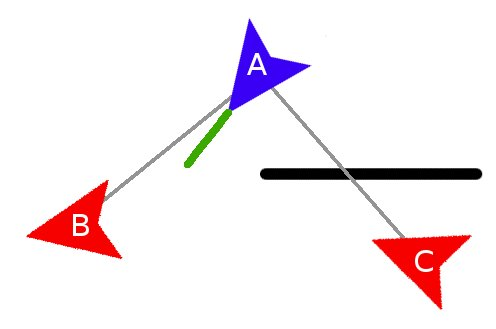
\includegraphics[width=80mm,height=53mm]{images/detection}
	\caption[Zauważanie przeciwnika]{Zauważanie przeciwnika: Najbliższym przeciwnikiem jednostki A jest jednostka B. Jednostka C nie jest analizowana, ponieważ znajduje się za ścianą. Zielona linia to linia sprawdzająca ew. kolizje dla jednostki A\label{detectionImage}}
\end{center}
\end{figure}

Algorytm zauważania przeciwnika jest zaimplementowany w metodzie \emph{closestSeenOpponent} klasy Game.Entity. Zwraca on referencję do najbliższego przeciwnika, będącego w zasięgu wzroku. Algorytm iteruje po liście przeciwników, dokonując szeregu sprawdzeń tylko dla tych jednostek, które jeszcze żyją. Tzw. \emph{dłuższy dystans} obliczany jest między pozycją obserwującej jednostki a pozycją potencjalnego przeciwnika. \emph{Krótszy dystans} obliczany jest między końcem linii sprawdzającej ew. kolizje dla jednostki obserwującej a pozycją potencjalnego przeciwnika (rysunek \ref{detectionImage}). Jeżeli \emph{krótszy dystans} jest rzeczywiście mniejszy od \emph{dłuższego dystansu}, to oznacza to, że przeciwnik jest przed jednostką obserwującą\footnote{jednostki będące za plecami jednostki obserwującej są ignorowane}. Jeżeli dystans pomiędzy jednostkami jest większy od zasięgu wzroku lub jest większy niż zapamiętany dystans do aktualnego celu, to taki przeciwnik jest ignorowany. Jeżeli jednak odległości są mniejsze, a przeciwnik nie znajduje się za jakąkolwiek ścianą, to oznaczamy go za cel i zapamiętujemy nowy, aktualny dystans do celu. Pseudokod algorytmu jest zapisany w~listingu \ref{detectionCode}.

\begin{table}
\begin{center}
\begin{lstlisting}
	cel = null
	dystans_do_celu = ja.zasieg_wzroku
	DLA KAZDEGO przeciwnik z lista_przeciwnikow WYKONUJ
		JEZELI przeciwnik.nie_zyje TO wykonaj_nastepna_iteracje
		dluzszy_dystans = oblicz_dystans (ja.pozycja, przeciwnik.pozycja)
		krotszy_dystans = oblicz_dystans (ja.koniec_promienia_kolizji, przeciwnik.pozycja)
		JEZELI krotszy_dystans < dluzszy_dystans ORAZ krotszy_dystans < dystans_do_celu TO
			JEZELI lista_scian_na_drodze (ja.pozycja, przeciwnik.pozycja) JEST PUSTA TO
				cel = przeciwnik
				dystans_do_celu = krotszy_dystans		
	ZWROC cel	
\end{lstlisting}
\caption {Pseudokod algorytmu zauważania przeciwnika}
\label{detectionCode}
\end{center}
\end{table}

\subsection{Podążanie jednostek w linii}

\begin{figure}
\begin{center}
	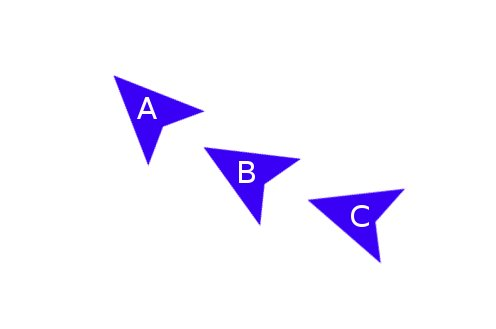
\includegraphics[width=80mm,height=53mm]{images/followEntity}
	\caption[Podążanie jednostek w linii]{Podążanie jednostek w linii: Jednostka A jest liderem. Z jednostką A, w określonym odstępie porusza się jednostka B, natomiast za jednostką B porusza się jednostka C\label{followEntityImage}}
\end{center}
\end{figure}

Antyterroryści w grze symulacyjnej poruszają się w szyku liniowym (rysunek \ref{followEntityImage}). Taka kolumna zaatakowana bezpośrednio od przodu lub od tyłu ma najmniejszą siłę ogniową. Linia zaatakowana od boku posiada bardzo dużą siłę ogniową, bowiem antyterroryści nie zasłaniają sobie na wzajem celu. Algorytm podążania w linii jest zaimplementowany w metodzie \emph{followEntity} klasy Game.Antiterrorist. Próbuje on dla danej jednostki znaleźć przyjazną jednostkę, która ją poprzedza i nie zginęła. Jeżeli taka jednostka nie zostanie znaleziona, to oznacza to, że dana jednostka jest liderem i należy zmienić jej stan na \emph{follow path}. W przeciwnym wypadku dana jednostka wylicza i podąża do współrzędnych celu, które są iloczynem odległości podążania oraz różnicy aktualnej pozycji znalezionego sprzymierzeńca i jego wektora prędkości. Pseudokod algorytmu jest zapisany w~listingu \ref{followEntityCode}.

\begin{table}
\begin{center}
\begin{lstlisting}
	indeks = ja.indeks_w_grupie
	POWTARZAJ
		indeks = indeks - 1
		sprzymierzeniec = sprzymierzency[indeks]
	DOPOKI (ISTNIEJE(sprzymierzeniec) ORAZ sprzymierzeniec.nie_zyje)
	JEZELI (NIE_ISTNIEJE(sprzymierzeniec)) TO
		ja.jestLiderem = PRAWDA
		ja.zmien_stan('follow path')
	WPP
		ja.jednostka_cel = sprzymierzeniec

	ja.pozycja_celu = (sprzymierzeniec.wektor_pozycji - sprzymierzeniec.wektor_predkosci) * ja.odleglosc_podazania
	ja.seek()
\end{lstlisting}
\caption {Pseudokod algorytmu podążania za jednostką}
\label{followEntityCode}
\end{center}
\end{table}

\subsection{Atakowanie jednostki}
Atak na wrogą jednostkę jest poprzedzany obserwacją, która przeprowadzana jest niezależnie od stanu, w jakim znajduje się aktualnie jednostka. Z tego algorytmu korzystają zarówno antyterroryści, jak i terroryści. Jest on zaimplementowany w~metodzie \emph{watchForEnemy} klasy Game.Entity. Na początku metoda korzysta z~algorytmu zauważania przeciwnika (rozdział \ref{detectionSubsection}). Jeżeli dana jednostka nie widzi w~danym momencie potencjalnego przeciwnika, a obecnie znajduje się w stanie \emph{attack}, to następuje przejście do stanu domyślnego tej jednostki. Jednak gdy przeciwnik został znaleziony, ale nie był wcześniej obserwowany, to dana jednostka rozpoczyna jego obserwację ustawiając czas do ataku na zdefiniowany w parametrach czas reakcji. Gdy jednak znaleziony przeciwnik jest już obserwowany i upłynie czas do ataku, to dana jednostka przechodzi do stanu \emph{attack}, jeżeli tylko nie ma przed sobą żadnych sprzymierzeńców stojących na linii ognia. Pseudokod algorytmu jest zapisany w listingu \ref{watchForEnemyCode}.

\begin{table}
\begin{center}
\begin{lstlisting}
	najblizszy_przeciwnik = znajdz_najblizszego_przeciwnika();
	JEZELI (NIE_ISTNIEJE(najblizszy_przeciwnik)) TO
		JEZELI (ja.aktualny_stan == 'attack')
			ja.pozycja_celu = null
			ja.zmien_stan_na_domyslny()
	WPP
		JEZELI (najblizszy_przeciwnik != ja.obserwowany_przeciwnik) TO
			ja.obserwowany_przeciwnik = najblizszy_przeciwnik
			ja.czas_do_ataku = ja.czas_reakcji
		WPP
			ja.czas_do_ataku = ja.czas_do_ataku - 1
			JEZELI (ja.czas_do_ataku < 0) TO
				JEZELI lista_sprzymierzencow_na_drodze (ja.pozycja, najblizszy_przeciwnik.pozycja) JEST PUSTA TO
					ja.jednostka_cel = najblizszy_przeciwnik
					ja.zmien_stan('attack')									
\end{lstlisting}
\caption {Pseudokod algorytmu obserwowania wroga}
\label{watchForEnemyCode}
\end{center}
\end{table}

Realizacja ataku polega na wystrzeliwaniu pocisku co określony interwał czasowy. Jeżeli upływa czas do kolejnego strzału, to tworzona jest nowa instancja pocisku, którego pozycja i orientacja są zgodne z odpowiednikami u strzelca. Obiekt pocisku wykonuje metodę \emph{move}, która sprawdza, czy pocisk nie trafił w ścianę lub jednostkę. W tym drugim przypadku zadawane są obrażenia zgodnie z energią, jaką posiadał pocisk w momencie trafienia. Pseudokod algorytmu ataku jest zapisany w listingu \ref{attackCode}.

\begin{table}
\begin{center}
\begin{lstlisting}
	ja.uaktualnij_pozycje_cel()
	ja.seek()				
	JEZELI (ja.czas_do_strzalu < 0) TO
		ja.czas_do_strzalu = ja.czas_miedzy_strzalami
		strzelec = ja
		UTWROZ('pocisk', strzelec)
	ja.czas_do_strzalu = ja.czas_do_strzalu - 1;
\end{lstlisting}
\caption {Pseudokod algorytmu atakowania wroga}
\label{attackCode}
\end{center}
\end{table}

\section{Parametryzacja}

Antyterroryści i terroryści w grze symulacyjnej współdzielą część metod oraz parametrów, które dziedziczą z klasy Game.Entity. Jednakże część parametrów wpływających na przebieg symulacji ma u nich różne wartości. Stroną faworyzowaną są tutaj antyterroryści, u których zakłada się, że są lepiej wyposażeni (np. większa szybkostrzelność broni, kamizelki kuloodporne) oraz są lepiej wyszkoleni (np. szybciej potrafią zareagować na pojawienie się przeciwnika). Dzięki takiej parametryzacji mniej liczebny odział antyterrorystów ma wyrównane szanse walki z liczniejszymi terrorystami. Tabela \ref{parameters} przedstawia porównanie wartości wybranych parametrów jednostek.

\begin{table}
\begin{center}
\begin{tabular}{|p{0.5\textwidth} | p{0.2\textwidth} p{0.2\textwidth}|}
\hline
Parametr & Antyterrorysta & Terrorysta\\\hline
	healthPoints (punkty życia) & 150 & 100\\\hline
	reactionTimeMax (czas reakcji) & 20 & 25\\\hline
	shootInterval (czas między strzałami) & 10 & 15\\\hline
	checkLocationTimeMax (czas na sprawdzenie lokacji) & 100 & 1000\\\hline
	maxSpeed (maksymalna prędkość) & 0.025 & 0.020\\
\hline
\end{tabular}
\caption {Porównanie parametrów antyterrorysty i terrorysty\label{parameters}}
\end{center}
\end{table} 

